
\chapter{Introduction}    % For a new chapter (works in book and report class)
\subsubsection{Disturbances and uncertainties}
% page1
% -------------------------------------

    The key word \textit{Robust} suggests that we are taking uncertainties into account. The model of the plant is as following:

%Graph
\begin{figure}[htbp]
    \centering
    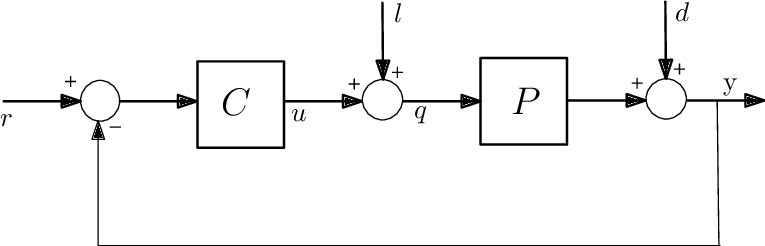
\includegraphics[width=\textwidth]{images/1.png} % Adjust width as needed
    \caption{A general control plant with additive disturbances \textit{l} and \textit{d}}
    \label{fig:graph_label}
\end{figure}


The general nonlinear state-space representation of the system is:

\begin{equation}
    \begin{cases}
    \dot{x}(t) = f(x(t), u(t)) \\
    y(t) = g(x(t), u(t))
    \end{cases}
\end{equation}
Where:
\begin{itemize}
    \item $x(t)$ is the state vector,
    \item $u(t)$ is the input vector,
    \item $y(t)$ is the output vector,
    \item $f(\cdot)$ is a nonlinear function describing the system dynamics,
    \item $g(\cdot)$ is a nonlinear function describing the output equation.\\
\end{itemize}

%page 2
%--------------------------------------------------
    \textbf{The first step} of any control problem is typically \textbf{derivation of mathematical model of the plant.} This step is the most crucial step, because if we drive the model by applying first principles of physics, we are likely to adopt approximated models, adopting simplifying assumptions, e.g. rigid body assumption etc. Further, the value of the physical parameters involved in the equations, such as friction coefficient, are not exactly known. Such approximations introduce errors and uncertainty in the mathematical description of the plant to be studied and controlled.

% page 3
% -----------------------------------------------------
    This fact is critical, since standard approaches to controller design are model-based; that is, the controller design has a strong dependency on the mathematical models used to describe the plant to be studied and controlled.


\begin{center}
$\textit{\textbf{Neglecting some physical details}} \equiv \textit{\textbf{Neglecting some state variables}}$
\end{center}

    For example, for modelling a robotic arm, generally, rigidity is assumed for the joints. Nevertheless, in fast movements  this assumption does not hold anymore, and the model does not predict the real performance of the robot, neglecting some state variables. Further, in some applications, we are not even aware of the phenomenon or phenomena that is being neglected. 

\subsubsection{Counter act for disturbances and uncertainties}

\begin{itemize}
    \item \textbf{First counter act}  These uncertainties and disturbances directly affect the controller design in the time domain, since the feedback gain and observer are directly calculated by solving algebraic equations including physical parameters with uncertainties. Nontheless, In frequency domain, the design of the controller is less affected by these uncertainties. 

    This does not mean that \textit{Transfer Function} is not affected by uncertainties of the parameters, because not considering some phenomona leads to the transfer function having less poles or zeros and because the uncertainty of the parameters affect the coefficients of the complex variables, being \textit{s} or \textit{z}. In the frequency domain design, we design the controller based on the frequency response of the system, considering cutting frequencies that reject high-frequency and low-frequency disturbances. In addition, by considering phase-margin and gain-margin, some margin for disturbances and uncertainties are taken into accoutn.

\textbf{Question to be answered: the sensitivity function is high-pass filter, meaning that the high frequency phenomenon, on the other-hand T is a low-pass filter, if the plant is designed for having a fast rising time, high-frequency phenomena also passes T.}

    \item \textbf{Second counter act}: Optimization problems in state-space where introduced to tackle this problem.
    \item \textbf{Third counter act}: Optimization problem, in state space, is combined with the concept of robustness, in frequency space, which is called $H_{\infty}$. 
\end{itemize}


\subsubsection{What is going to be discussed in this course}
    In the first part of this course, we are going to learn how to learn from the mapping from the input to the output of the system, extracting a \textbf{mathematical model} for the plant. Further, it elaborates on this data to drive also a \textbf{discription for uncertainty}. These, together, can be used for \textbf{robust controller design} in a model-based approach.

    In the second step, the aim is to design a controller directly from the data, without the intervention of the model.


\begin{factbox}[Professor's Quote]

    In conclusion, even if the physical model is very precise, at some point, in order to measure the parameters used in the physical models, it is required to do some experimental measurements, subjected to noise, introducing uncertainties to our model.\newline \newline
    If these uncertainties are not taken into account, the controller will not have a good performance when implemented physically, and it is going to work only in simulations. \newline \newline
    There are many approaches to tackle this problem. Here, in the first part of the course, we will focus on \textbf{System Identification}, which is another modelling paradigm. In this paradigm, we learn the mathematical model of the system to be controlled by using experimentally collected data. Not only do we introduce what \textit{System identification} is and what are the possible approached, but maintly to focus on \textbf{\textit{Set-membership Identification Technique}} that allow us to learn the model of the system, and drive information about how the uncertainty is affecting out model; this is used to design a controller in a robust manner. Robust controller designed can be directly applied to the real physical plants.  \newline \newline
    
    In the second part of the course, we shift our paradigm again. In this part, assuming that the collected data represents the behavior of the mapping between the input and output, we try to design the controller directly from the data, called  \textbf{Direct Data-Driver Controller Design}. \newline \newline
    
\end{factbox}

